% !TeX program = xelatex
\documentclass[a4paper,10pt]{article}

% ============================================================================
% សន្លឹកកិច្ចការសិស្សបំពេញចន្លោះ ស-ខ្មៅ និងប្លង់ក្ដារខៀន/ចម្លើយគ្រូ (គ្មាន LCD / គ្មានកន្ត្រៃ)
% មេរៀនទី៥ (៤.៣)៖ របៀបផ្សេងៗក្នុងការដាក់កន្សោមជាផលគុណកត្តា — ត្រូវគ្នានឹង LS_Plan_ALG58.tex
% ============================================================================
\usepackage[a4paper, left=1.0cm, right=1.0cm, top=0.75cm, bottom=1.00cm, footskip=0.52cm]{geometry}
\usepackage{amsmath}
\usepackage{unicode-math}
\usepackage{fontspec}
\usepackage{array, colortbl}
\usepackage[table]{xcolor}
\usepackage{enumitem}
\usepackage{pifont}
\usepackage{fancyhdr}
\usepackage{lastpage}
\usepackage{tikz}
\usepackage[most]{tcolorbox}
\usetikzlibrary{calc, arrows.meta, decorations.pathreplacing, positioning, babel}

\makeatletter
\let\@expl@@@mark@update@singlecol@structures@@\relax
\makeatother

\providecommand{\NGSFindFonts}{%
  \IfFileExists{C:/Windows/Fonts/cambria.ttc}{%
    \def\NGSSysPath{C:/Windows/Fonts/}%
    \def\NGSUserPath{C:/Users/KIT/AppData/Local/Microsoft/Windows/Fonts/}%
  }{%
    \IfFileExists{./fonts/KhmerOSsiemreap.ttf}{\def\NGSSysPath{./fonts/}\def\NGSUserPath{./fonts/}}{%
    \IfFileExists{../fonts/KhmerOSsiemreap.ttf}{\def\NGSSysPath{../fonts/}\def\NGSUserPath{../fonts/}}{%
    \IfFileExists{../../fonts/KhmerOSsiemreap.ttf}{\def\NGSSysPath{../../fonts/}\def\NGSUserPath{../../fonts/}}{%
    \IfFileExists{../../../fonts/KhmerOSsiemreap.ttf}{\def\NGSSysPath{../../../fonts/}\def\NGSUserPath{../../../fonts/}}{%
    \IfFileExists{../../../../fonts/KhmerOSsiemreap.ttf}{\def\NGSSysPath{../../../../fonts/}\def\NGSUserPath{../../../../fonts/}}{%
    \IfFileExists{../../../../../fonts/KhmerOSsiemreap.ttf}{\def\NGSSysPath{../../../../../fonts/}\def\NGSUserPath{../../../../../fonts/}}{%
    \IfFileExists{../../../../../../fonts/KhmerOSsiemreap.ttf}{\def\NGSSysPath{../../../../../../fonts/}\def\NGSUserPath{../../../../../../fonts/}}{%
      \def\NGSSysPath{../../../../../../../fonts/}\def\NGSUserPath{../../../../../../../fonts/}%
    }}}}}}}%
  }%
}
\NGSFindFonts

\setmathfont[Path={\NGSSysPath}, FontIndex=1, Scale=1.02]{cambria.ttc}
\defaultfontfeatures{Ligatures=TeX}

\setmainfont[
  Path={\NGSUserPath}, Extension=.ttf, Script=Khmer,
  BoldFont={KhmerOSsiemreap}, BoldFeatures={FakeBold=1.8},
  ItalicFont={KhmerOSsiemreap}, ItalicFeatures={FakeSlant=0.25},
  BoldItalicFont={KhmerOSsiemreap}, BoldItalicFeatures={FakeBold=1.8, FakeSlant=0.25}
]{KhmerOSsiemreap}

\newfontfamily\muol[Path={\NGSUserPath}, Extension=.ttf, Script=Khmer]{KhmerOSmuollight}
\newfontfamily\TimesEn[Path={\NGSSysPath}, Extension=.ttf, BoldFont={timesbd}, ItalicFont={timesi}, BoldItalicFont={timesbi}]{times}
\newfontfamily\CalibriFont[Path={\NGSSysPath}, Extension=.ttf]{calibri}

\XeTeXlinebreaklocale "km"
\XeTeXlinebreakskip = 0pt plus 1pt minus 0.1pt

\definecolor{panelgray}{gray}{0.94}
\definecolor{headgray}{gray}{0.85}

\pagestyle{fancy}
\fancyhf{}
\renewcommand{\headrulewidth}{0pt}
\fancyfoot[L]{\fontsize{7.4pt}{9.5pt}\selectfont អនុវិទ្យាល័យព្រះក្រសាំង \en{|} គ្រូ៖ ហុក ប៊ុនថែន \en{|} មេរៀនទី៥ (៤.៣) របៀបផ្សេងៗនៃការដាក់ជាផលគុណកត្តា \en{|} ថ្ងៃសៅរ៍ ទី១២ ខែធ្នូ ឆ្នាំ២០២៦}
\fancyfoot[R]{\fontsize{7.8pt}{10pt}\selectfont ទំព័រ \en{\thepage\ / \pageref{LastPage}}}

\setlength{\parindent}{0pt}
\setlength{\parskip}{0pt}
\setlength{\tabcolsep}{4pt}

\newcommand{\en}[1]{{\TimesEn #1}}
\newcommand{\enbf}[1]{{\TimesEn\bfseries #1}}
\newcommand{\unit}[1]{\,\text{\en{#1}}}
\newcommand{\riel}{\,\text{៛}}
\newcommand{\cnum}[1]{\mbox{\fontsize{10pt}{12pt}\selectfont\ding{\numexpr181+#1\relax}}}
\newcommand{\chkbox}{\tikz[baseline=-0.15ex]\draw[black, line width=0.85pt, fill=white] (0,0) rectangle (0.24cm,0.24cm);}
\newcommand{\ansbox}[1][2.0cm]{\,\tikz[baseline=-0.65ex]\draw[black, line width=0.65pt, fill=white] (0,0) rectangle (#1, 0.42cm);\,}
\newcommand{\dotline}[1][2.2cm]{\makebox[#1]{\dotfill}}

\newcommand{\pagebanner}[2]{%
  \begin{tcolorbox}[
    enhanced, sharp corners, colback=headgray, colframe=black,
    boxrule=1.05pt, boxsep=1pt, top=2.5pt, bottom=2.5pt, left=6pt, right=6pt,
    after skip=3.5pt
  ]
    {\muol\fontsize{9.0pt}{13.2pt}\selectfont #1}\hfill{\fontsize{8.0pt}{11.2pt}\selectfont\textbf{#2}}
  \end{tcolorbox}%
}

\newcommand{\secstrip}[2]{%
  \vspace{3pt}%
  \begin{tcolorbox}[
    enhanced, sharp corners, colback=panelgray, colframe=black,
    boxrule=0.8pt, boxsep=0.8pt, top=2pt, bottom=2pt, left=5pt, right=5pt,
    after skip=3pt
  ]
    {\muol\fontsize{8.5pt}{12.2pt}\selectfont #1}\hfill{\fontsize{7.8pt}{10.8pt}\selectfont\textit{#2}}
  \end{tcolorbox}%
}

\newcolumntype{L}[1]{>{\raggedright\arraybackslash}p{#1}}
\newcolumntype{C}[1]{>{\centering\arraybackslash}p{#1}}

\begin{document}
\fontsize{9.5pt}{14.5pt}\selectfont

% ============================================================================
% ទំព័រទី ១៖ សន្លឹកកិច្ចការសិស្ស (ផ្នែកមុខ៖ E1 -> E2 -> E3)
% ============================================================================
\pagebanner{សន្លឹកកិច្ចការសិស្ស \enbf{(}៥\enbf{.}៤\enbf{.}៣ របៀបផ្សេងៗនៃការដាក់ជាកត្តា\enbf{)} \enbf{--} ផ្នែកមុខ}{ថ្នាក់ទី៨ \en{|} ទំ.៧១--៧២}

\begin{tcolorbox}[
  enhanced, sharp corners, colback=white, colframe=black,
  boxrule=0.8pt, boxsep=1.5pt, top=3.5pt, bottom=3.5pt, left=5pt, right=5pt,
  after skip=4pt
]
  \fontsize{9.0pt}{13.0pt}\selectfont
  \textbf{ឈ្មោះសិស្ស៖} \dotline[4.3cm] \quad
  \textbf{សមាជិកក្រុម៖} \dotline[4.3cm] \quad
  \textbf{ថ្នាក់ទី៖} ៨\dotline[0.9cm] \quad
  \textbf{ក្រុមទី៖} \dotline[1.0cm]
\end{tcolorbox}

% --- E1 Engage ---
\secstrip{ផ្នែកទី ១ \enbf{(E1 - Engage)} ៖ បេសកកម្មដាក់ជាផលគុណកត្តាឱ្យអស់លទ្ធភាព}{រយៈពេល ៣ នាទី (គូស \ding{51} ក្នុង \chkbox)}

\begin{tcolorbox}[
  enhanced, sharp corners, colback=white, colframe=black,
  boxrule=0.8pt, boxsep=2.5pt, top=4pt, bottom=4pt, left=6pt, right=6pt
]
  គេចង់ដាក់ពហុធា $A = x^3 - 2x^2 - 4x + 8$ (ទំ.៧១) ជាផលគុណកត្តាឱ្យអស់លទ្ធភាព ។ តើអ្នកណាដាក់អស់លទ្ធភាព?\\[3pt]
  \chkbox\ \textbf{សិស្ស ក៖} $A = x^2(x - 2) - 4(x - 2) = (x - 2)(x^2 - 4)$ \qquad
  \chkbox\ \textbf{សិស្ស ខ៖} $A = (x - 2)(x - 2)(x + 2) = (x - 2)^2(x + 2)$\\[3pt]
  $\bullet$ \textbf{ពិនិត្យ៖} ព្រោះកត្តា $x^2 - 4$ គឺជាផលដកពីរការេ $x^2 - 2^2 =$ \dotline[3.2cm] ។
\end{tcolorbox}

\vspace{3pt}

% --- E2 Explore ---
\secstrip{ផ្នែកទី ២ \enbf{(E2 - Explore)} ៖ បំពេញការេទ្វេធា បំបែកតួកណ្ដាល និងផ្ដុំតួ (ទំ.៧១--៧២)}{រយៈពេល ១១ នាទី}

\textbf{សកម្មភាព ១ (\en{E2-A} — ៦ នាទី)៖ វិធីបំពេញការេទ្វេធា និងបំបែកតួកណ្ដាល (ទំ.៧១ ឧទាហរណ៍ទី ១ និងទី ៣)}

\begin{tcolorbox}[
  enhanced, sharp corners, colback=white, colframe=black,
  boxrule=0.8pt, boxsep=2.5pt, top=4pt, bottom=4pt, left=6pt, right=6pt
]
  $\bullet$ \textbf{១) ឧទាហរណ៍ទី ១ (បំពេញការេ)៖} $A = x^2 - 2x - 8 = (x^2 - 2x + 1) - 1 - 8 = (x - 1)^2 - 3^2 =$ \ansbox[3.8cm]\\[3pt]
  $\bullet$ \textbf{២) ឧទាហរណ៍ទី ៣ (បំបែកតួកណ្ដាល)៖} $F = 3x^2 - 4x - 7 = 3x^2 + 3x - 7x - 7 = 3x(x+1) - 7(x+1) =$ \ansbox[3.6cm]
\end{tcolorbox}

\vspace{4pt}
\textbf{សកម្មភាព ២ (\en{E2-B} — ៥ នាទី)៖ វិធីបន្ថែម-ដកតួកណ្ដាល និងផ្ដុំតួ ៤ តួ (ទំ.៧១--៧២)}

\begin{tcolorbox}[
  enhanced, sharp corners, colback=white, colframe=black,
  boxrule=0.8pt, boxsep=2.5pt, top=4pt, bottom=4pt, left=6pt, right=6pt
]
  $\bullet$ \textbf{១) ឧទាហរណ៍ទី ២ (ទំ.៧១)៖} $E = 9t^4 - 28t^2 + 16 = (3t^2 - 4)^2 - (2t)^2 =$ \ansbox[4.8cm]\\[3pt]
  $\bullet$ \textbf{២) លំហាត់គំរូផ្ដុំតួ (ទំ.៧១--៧២)៖} $A = x^3 - 2x^2 - 4x + 8 = x^2(x-2) - 4(x-2) = (x-2)(x^2-4) =$ \ansbox[4.2cm]
\end{tcolorbox}

\vfill

% --- E3 Explain ---
\secstrip{ផ្នែកទី ៣ \enbf{(E3 - Explain)} ៖ សង្ខេបយុទ្ធវិធីទាំង ៣ និងធនាគារហេតុផល \enbf{B\&W}}{រយៈពេល ៦ នាទី}

\begin{tcolorbox}[
  enhanced, sharp corners, colback=white, colframe=black,
  boxrule=0.85pt, boxsep=2.5pt, top=4pt, bottom=4pt, left=6pt, right=6pt
]
  $\bullet$ \textbf{១) បំពេញការេទ្វេធា៖} បម្លែងជាទម្រង់ \ansbox[3.4cm] រួចប្រើរូបមន្ត $U^2 - V^2 = (U-V)(U+V)$\\[4pt]
  $\bullet$ \textbf{២) បំបែកតួកណ្ដាល ($ax^2+bx+c$)៖} រកពីរចំនួន $p, q$ ដែល $p + q =$ \ansbox[1.8cm] និង $p \cdot q =$ \ansbox[2.0cm]\\[4pt]
  $\bullet$ \textbf{៣) ផ្ដុំតួ ៤ តួ៖} ផ្ដុំជា $(2\text{ តួ}) + (2\text{ តួ})$ ដើម្បីរកកត្តារួម ឬផ្ដុំជា $(3\text{ តួ}) - (1\text{ តួ})$\\[4pt]
  \tikz\draw[black, dashed, line width=0.6pt] (0,0) -- (\linewidth,0);\\[3pt]
  \fontsize{8.8pt}{13.0pt}\selectfont
  \textbf{ធនាគារហេតុផល (\en{Warrant Bank})៖} \quad
  \cnum{1} បន្ថែម $+h^2$ ត្រូវដក $-h^2$ វិញ \quad
  \cnum{2} ផ្ទៀងទាំង $p+q=b$ និង $pq=ac$\\
  \cnum{3} ដាក់វង់ក្រចកក្រោយ $(-)$ ត្រូវប្ដូរសញ្ញាខាងក្នុង \quad
  \cnum{4} ពិនិត្យបំបែកកត្តាដឺក្រេទី ២ ឬទី ៣ បន្តឱ្យអស់លទ្ធភាព
\end{tcolorbox}

% ============================================================================
% ទំព័រទី ២៖ សន្លឹកកិច្ចការសិស្ស (ផ្នែកខាងខ្នង៖ E4 -> E5 -> កិច្ចការផ្ទះ)
% ============================================================================
\clearpage
\pagebanner{សន្លឹកកិច្ចការសិស្ស \enbf{(}៥\enbf{.}៤\enbf{.}៣ របៀបផ្សេងៗនៃការដាក់ជាកត្តា\enbf{)} \enbf{--} ផ្នែកខ្នង}{ថ្នាក់ទី៨ \en{|} ទំ.៧១--៧២, ៧៤}

% --- E4 Elaborate ---
\secstrip{ផ្នែកទី ៤ \enbf{(E4 - Elaborate)} ៖ លំហាត់គំរូពង្រីក (ទំ.៧១--៧២ និង ទំ.៧៤ \enbf{\#16})}{រយៈពេល ១០ នាទី}

\begin{tcolorbox}[
  enhanced, sharp corners, colback=white, colframe=black,
  boxrule=0.8pt, boxsep=2.5pt, top=4pt, bottom=4pt, left=6pt, right=6pt
]
  \textbf{១) លំហាត់គំរូ $B, C, D$ (ទំ.៧១--៧២)៖}\\[3pt]
  \hspace*{0.3cm}$\bullet$ $B = 4x^2 + y^2 - b^2 - 4xy = (4x^2 - 4xy + y^2) - b^2 = (2x - y)^2 - b^2 =$ \ansbox[4.8cm]\\[3pt]
  \hspace*{0.3cm}$\bullet$ $C = (a - 4)(y + 2) - (a - 4)(3y + 2) =$ \ansbox[3.6cm]\\[3pt]
  \hspace*{0.3cm}$\bullet$ $D = x^3(x + 1) + y^3(x + 1) = (x + 1)(x^3 + y^3) =$ \ansbox[5.2cm]\\[4pt]
  \textbf{២) លំហាត់ \en{\#16} ក, ខ (ទំ.៧៤)៖} $A = b^2 + 8b + 15 = (b^2 + 8b + 16) - 1 = (b + 4)^2 - 1^2 =$ \ansbox[3.8cm]\\[4pt]
  \textbf{ឆ្លុះបញ្ចាំង (\en{EIA Looking-Back})៖} ហេតុអ្វី $-4x + 8 = -4(x - 2)$ មិនមែន $-4(x + 2)$? \dotline[4.8cm] ។
\end{tcolorbox}

\vspace{4pt}

% --- E5 Evaluate ---
\secstrip{ផ្នែកទី ៥ \enbf{(E5 - Evaluate)} ៖ ប្រតិបត្តិ (ទំ.៧៤) សំណួរវិនិច្ឆ័យ \enbf{A--D} និងសំបុត្រចេញ}{រយៈពេល ១០ នាទី}

\begin{tcolorbox}[
  enhanced, sharp corners, colback=white, colframe=black,
  boxrule=0.8pt, boxsep=2.5pt, top=4pt, bottom=4pt, left=6pt, right=6pt
]
  \textbf{១) ប្រតិបត្តិជាក្រុម (ទំ.៧៤ \en{\#12, \#15, \#16})៖}\\[3pt]
  \hspace*{0.3cm}$\bullet$ \en{\#12} ច៖ $8ax - bx + 8ay - by =$ \ansbox[3.6cm] \qquad
  \en{\#15} ក៖ $x^2 + 3x + 2 =$ \ansbox[3.4cm]\\[3pt]
  \hspace*{0.3cm}$\bullet$ \en{\#15} ខ៖ $3x^2 + 14x + 8 =$ \ansbox[3.6cm] \qquad\qquad
  \en{\#16} គ ($B$)៖ $x^2 + 4x + 3 =$ \ansbox[3.4cm]\\[4pt]
  \textbf{២) បិទបេសកកម្ម \en{E1}៖} សិស្ស \dotline[1.1cm] ត្រឹមត្រូវ ព្រោះ $A = (x - 2)(x^2 - 4) =$ \ansbox[3.8cm] ។
\end{tcolorbox}

\vspace{4pt}

\begin{tcolorbox}[
  enhanced, sharp corners, colback=white, colframe=black,
  boxrule=0.85pt, boxsep=2.5pt, top=4pt, bottom=4pt, left=6pt, right=6pt
]
  \textbf{៣) សំណួរវិនិច្ឆ័យ \en{A--D} (ដាក់ត្រីធា $x^2 - 5x + 6$ ជាផលគុណកត្តា — គូសរង្វង់ រួចលើកម្រាមដៃ ១--៤)៖}\\[3pt]
  \textbf{\en{A.}} $(x - 6)(x + 1)$ \qquad\quad
  \textbf{\en{B.}} $(x + 2)(x + 3)$ \qquad\quad
  \textbf{\en{C.}} $(x - 2)(x - 3)$ \qquad\quad
  \textbf{\en{D.}} $(x - 5)(x + 6)$\\[4pt]
  \tikz\draw[black, dashed, line width=0.6pt] (0,0) -- (\linewidth,0);\\[3pt]
  \textbf{៤) សំបុត្រចេញ ៦០ វិនាទី (ទំ.៧៤ \en{\#12} ឆ)៖} $ax + ay - 2bx - 2by =$ \ansbox[4.2cm] ។
\end{tcolorbox}

\vfill

% --- Homework Box ---
\begin{tcolorbox}[
  enhanced, sharp corners, colback=panelgray, colframe=black,
  boxrule=0.9pt, boxsep=2.5pt, top=4pt, bottom=4pt, left=6pt, right=6pt
]
  {\muol\fontsize{8.8pt}{13pt}\selectfont កិច្ចការផ្ទះ \enbf{(}សៀវភៅគោល ទំ\enbf{.}៧៤ លេខ ១២\enbf{,} ១៥\enbf{,} ១៦\enbf{)}}\\[3pt]
  $\bullet$ \textbf{១) ទំ.៧៤ \en{\#12} ង និង \en{\#16} គ ($C$)៖} ដាក់ជាផលគុណកត្តា $(y - 8)(4y - 1) + y^2 - 8y$ និង $C = 4x^2 - 8x + 3$ ។\\[2pt]
  $\bullet$ \textbf{២) ទំ.៧៤ \en{\#15} ឃ, ង, ជ៖} ដាក់ជាផលគុណកត្តា $2x^2 + 15x + 7$, $14a^2 + 18a - 20$ និង $6x^2 + 5x + 1$ ។
\end{tcolorbox}

% ============================================================================
% ទំព័រទី ៣៖ ទំព័រគ្រូបង្រៀន — ប្លង់ក្ដារខៀន ៣ ផ្នែក (គ្មាន LCD) និងចម្លើយផ្ទៀងផ្ទាត់រហ័ស
% ============================================================================
\clearpage
\pagebanner{ទំព័រគ្រូបង្រៀន ៖ ប្លង់ក្ដារខៀន \enbf{(}គ្មាន \enbf{LCD)} និងចម្លើយផ្ទៀងផ្ទាត់រហ័ស}{៥.៤.៣ របៀបផ្សេងៗនៃការដាក់ជាកត្តា (\en{ALG58})}

\secstrip{១. គំរូប្លង់បែងចែកក្ដារខៀន ៣ ផ្នែក សម្រាប់ថ្នាក់រៀនគ្មាន \enbf{LCD}}{សម្រាប់គ្រូប្រើដីស/ហ្វឺត}

\begin{center}
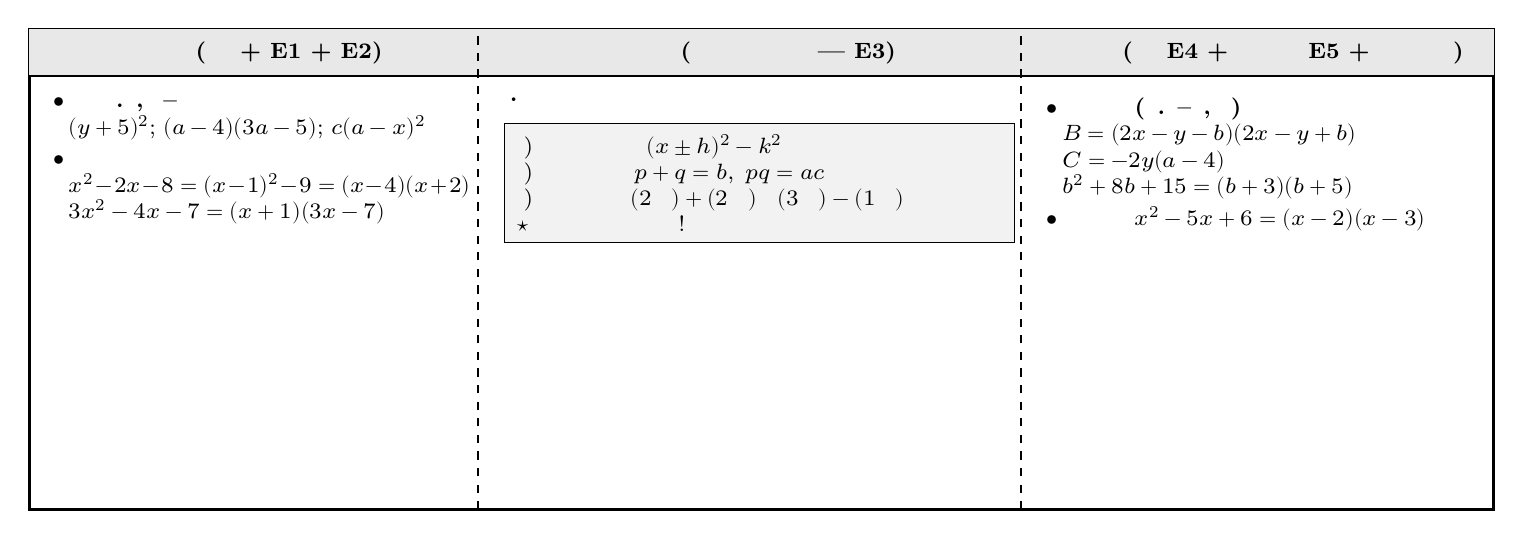
\begin{tikzpicture}[x=1cm, y=1cm, every node/.style={font=\footnotesize, text=black}]
  \draw[black, line width=1.1pt] (0,0) rectangle (18.6,6.1);
  \fill[gray!18] (0,5.50) rectangle (18.6,6.1);
  \draw[black, line width=0.7pt] (0,5.50) -- (18.6,5.50);
  \draw[black, dashed, line width=0.75pt] (5.7,0) -- (5.7,6.1);
  \draw[black, dashed, line width=0.75pt] (12.6,0) -- (12.6,6.1);

  \node at (2.85,5.80) {\textbf{ផ្នែកឆ្វេង (កំណែ + \en{E1} + \en{E2})}};
  \node at (9.15,5.80) {\textbf{ផ្នែកកណ្ដាល (ខ្លឹមសារគោលរក្សាទុក — \en{E3})}};
  \node at (15.60,5.80) {\textbf{ផ្នែកស្ដាំ (គំរូ \en{E4} + ប្រតិបត្តិ \en{E5} + កិច្ចការផ្ទះ)}};

  % Left zone
  \node[anchor=north west, text width=5.3cm] at (0.18,5.35) {
    $\bullet$ \textbf{កំណែ ទំ.៧០, ៧៣--៧៤៖}\\
    \hspace*{0.2cm}$(y+5)^2$; $(a-4)(3a-5)$; $c(a-x)^2$\\[2pt]
    $\bullet$ \textbf{បំពេញការេ និងបំបែកតួកណ្ដាល៖}\\
    \hspace*{0.2cm}$x^2-2x-8 = (x-1)^2-9 = (x-4)(x+2)$\\
    \hspace*{0.2cm}$3x^2-4x-7 = (x+1)(3x-7)$
  };

  % Center zone
  \node[anchor=north west, text width=6.5cm] at (5.90,5.35) {
    {\muol\fontsize{8.2pt}{12pt}\selectfont ៤\enbf{.}៣ យុទ្ធវិធីទាំង ៣ ក្នុងការដាក់ជាកត្តា}\\[3pt]
    \begin{tcolorbox}[enhanced, sharp corners, colback=gray!10, colframe=black, boxrule=0.6pt, boxsep=1.5pt, left=3pt, right=3pt, top=2pt, bottom=2pt]
      ១) បំពេញការេទ្វេធា៖ $(x\pm h)^2 - k^2$\\
      ២) បំបែកតួកណ្ដាល៖ $p+q=b,\ pq=ac$\\
      ៣) ផ្ដុំតួ ៤ តួ៖ $(2\text{ តួ})+(2\text{ តួ})$ ឬ $(3\text{ តួ})-(1\text{ តួ})$\\
      $\star$ បំបែកបន្តរហូតអស់លទ្ធភាព!
    \end{tcolorbox}
  };

  % Right zone
  \node[anchor=north west, text width=5.6cm] at (12.80,5.35) {
    $\bullet$ \textbf{លំហាត់គំរូ (ទំ.៧១--៧២, ៧៤)៖}\\
    \hspace*{0.2cm}$B = (2x-y-b)(2x-y+b)$\\
    \hspace*{0.2cm}$C = -2y(a-4)$\\
    \hspace*{0.2cm}$b^2+8b+15 = (b+3)(b+5)$\\[2pt]
    $\bullet$ \textbf{វិនិច្ឆ័យ៖} $x^2-5x+6 = (x-2)(x-3)$
  };
\end{tikzpicture}
\end{center}

\secstrip{២. ចម្លើយផ្ទៀងផ្ទាត់រហ័សសម្រាប់សន្លឹកកិច្ចការសិស្ស \enbf{(}ទំព័រ ១ និង ទំព័រ ២\enbf{)}}{\en{Answer Key}}

\begin{tcolorbox}[
  enhanced, sharp corners, colback=white, colframe=black,
  boxrule=0.8pt, boxsep=2.5pt, top=4pt, bottom=4pt, left=6pt, right=6pt
]
  $\bullet$ \textbf{ផ្នែក \en{E1}៖} សិស្ស ខ ត្រឹមត្រូវ $(x-2)^2(x+2)$ ព្រោះ $x^2-4 = (x-2)(x+2)$ អាចបំបែកបន្តទៀតបាន ។\\[2pt]
  $\bullet$ \textbf{ផ្នែក \en{E2}៖} សកម្មភាព ១៖ $(x-4)(x+2)$; $(x+1)(3x-7)$ ។ សកម្មភាព ២៖ $(3t^2-2t-4)(3t^2+2t-4)$; $(x-2)^2(x+2)$ ។\\[2pt]
  $\bullet$ \textbf{ផ្នែក \en{E4}៖} ១) $(2x-y-b)(2x-y+b)$; $-2y(a-4)$; $(x+1)(x+y)(x^2-xy+y^2)$; ២) $(b+3)(b+5)$ ។\\[2pt]
  $\bullet$ \textbf{ផ្នែក \en{E5}៖} ១) $(8a-b)(x+y)$; $(x+1)(x+2)$; $(3x+2)(x+4)$; $(x+1)(x+3)$; ២) សិស្ស ខ; ៣) \textbf{ជម្រើស \en{C}} ($(x-2)(x-3)$); ៤) $(x+y)(a-2b)$ ។
\end{tcolorbox}

\secstrip{៣. ចម្លើយលម្អិតនៃកិច្ចការផ្ទះ \enbf{(}បញ្ចប់មេរៀនទី៥ — សម្រាប់ផ្ទៀងមុនចូលមេរៀនទី៦\enbf{)}}{សៀវភៅគោល ទំ.៧៤}

\begin{tcolorbox}[
  enhanced, sharp corners, colback=white, colframe=black,
  boxrule=0.8pt, boxsep=2.5pt, top=4pt, bottom=4pt, left=6pt, right=6pt
]
  $\bullet$ \textbf{១) ទំ.៧៤ \en{\#12} ង និង \en{\#16} គ ($C$)៖} $(y-8)(4y-1)+y(y-8) = \mathbf{(y-8)(5y-1)}$; \quad $C = 4x^2-8x+3 = (2x-2)^2-1 = \mathbf{(2x-3)(2x-1)}$ ។\\[2pt]
  $\bullet$ \textbf{២) ទំ.៧៤ \en{\#15} ឃ, ង, ជ៖} ឃ) $2x^2+15x+7 = \mathbf{(2x+1)(x+7)}$; \ ង) $14a^2+18a-20 = \mathbf{2(7a-5)(a+2)}$; \ ជ) $6x^2+5x+1 = \mathbf{(2x+1)(3x+1)}$ ។
\end{tcolorbox}

\end{document}
